\documentclass[final]{svjour2}
\usepackage{graphicx}
\usepackage{rotating}
\usepackage{amssymb}
\usepackage{wrapfig}
\usepackage{subfig}
\usepackage{amsmath}
\usepackage{mathptmx}
\usepackage[numbers]{natbib}
\usepackage[table]{xcolor}
\usepackage{tabularx}
\usepackage{multirow}
\usepackage{booktabs}
\usepackage{threeparttable}
\usepackage{epstopdf}

\providecommand{\e}[1]{\ensuremath{\times 10^{#1}}}
\renewcommand{\thefootnote}{\alph{footnote}}

\providecommand{\p}[1]{\phantom{#1}}

%\usepackage[nofighead,nomarkers]{endfloat}
\makeatletter
\journalname{Journal of Low Temperature Physics}
%%%%%%%%%%%%%%%%%%%%%%%%%%%%%% Textclass specific LaTeX commands.


%%%%%%%%%%%%%%%%%%%%%%%%%%%%%% User specified LaTeX commands.
\bibpunct{}{}{,}{s}{}{,}

\begin{document}

\newcommand{\hdblarrow}{H\makebox[0.9ex][l]{$\downdownarrows$}-}
\title{Sub-Kelvin Thermal Conductivity and Radioactivity of Some Useful Materials in Low Background Cryogenic Experiments}

\author{N. Kellaris \and M. Daal \and E. Kramer \and M. Epland \and M. Pepin \and O. Kamaev \and P. Cushman \and B. Sadoulet \and N. Mirabolfathi \and S. Golwala \and M. Runyan}

\institute{Department of Physics, University of California, Berkeley\\ Berkeley, CA 94720, USA\\
\email{nicholaskellaris@berkeley.edu}}

\date{XX.XX.20XX}

\maketitle


\begin{abstract}
     We present measurements of the thermal conductivity from 0.05K to 1K, and radioactive contamination levels, for some thermally isolating materials. TiMet Ti 15-3-3-3, Mersen grade 2020 graphite, Vespel SP-1, Vespel SP-22, Vespel SCP-5000, Vespel SCP-5050, Graphlite CFRP, and a Kapton/epoxy composite are all investigated. Thermal conductivities were measured using a single-heater longitudinal heat flow method. Material radioactivity was determined for the materials at a low background counting facility using a high-purity gamma detector and GEANT4 Monte Carlo simulations.


\keywords{thermal conductivity, radioactivity, low temperature, 15-3-3-3, 15333, Vespel, SP-1, SP-22, SCP-5000, SCP-5050, graphite, AXM-5Q, 2020, POCO, Mersen, CFRP, Graphlite, Kapton}

\end{abstract}

\section{Introduction}
Low temperature detector experiments often require materials with low thermal conductivity and -- in the case of low background experiments such as dark matter and double-beta decay -- low radioactivity. A literature search often comes up short when it comes to sub-Kelvin thermal conductivity measurements, and low-level radioactivity is seldom mentioned. We present thermal conductivity and radioactivity data for some materials which may prove useful for cryogenic experiments. TiMet Ti 15-3-3-3, Mersen grade 2020 graphite, Vespel SP-1, Vespel SP-22, Vespel SCP-5000, Vespel SCP-5050, Graphlite CFRP, and a Kapton/epoxy composite were tested. Not all materials were tested for both thermal conductivity and radioactivity.

\section{Materials Tested}
Four types of DuPont Vespel polyimide were tested: SP-1, SP-22, SCP-5000, and SCP-5050.  Vespel SP-1 is unfilled polyimide, while SP-22 is filled polyimide base (SP-1) with 40\% graphite by weight. SCP-5000 and SCP-5050 are the newer analogs of SP-1 and SP-22 respectively; they have improved dimensional stability and strength over the SP series. All were purchased from Curbell Plastics.

Two grades of graphite were tested. Mersen grade 2020 is a nuclear grade graphite with grain sizes of 15$\mu$m and bulk density of 1.77g/cm$^3$. POCO AXM-5Q is a highly isotropic (5$\mu$m grain size) industrial grade graphite with a bulk density of 1.73g/cm$^3$.

We tested TIMETAL Ti 15-3-3-3, a meta-stable beta titanium alloy with composition 76Ti-15V-3Al-3Cr-3Sn by weight, and a superconducting transition at 3.89K. We tested 0.84 mil thick foil from Arnold Magnetic Technologies.

A pultruded carbon-fiber composite made by Avia Sport Composites -- called Graphlite -- was tested. This is a unidirectional material with fibers nearly uniformly oriented along the pultrusion axis. Thermal conductivity was measured for a 0.156 inch diameter rod of standard modulus material, parallel to the fiber axis.

The last material measured was a Kapton-epoxy composite provided by Tech-Etch. The sample was 1 mil epoxy adhesive (pre-cured) on a 1 mil Kapton sheet. Thermal conductivity was measured parallel to the plane of the sheet. This is the same material that Tech-Etch uses in its laminated flex-circuits.

\section{Radioactivity of Samples}
The radioactive contamination of our samples was determined for five long-lived radioisotopes: $^{238}$U, $^{232}$Th, $^{60}$Co, $^{40}$K, and $^{137}$Cs. Measurements were performed in the Soudan Underground Laboratory\footnotemark using Gopher -- a 2.075 kg high-purity Ge gamma detector. Gamma events were counted for up to 30 days for each sample, then modelled using GEANT4 Monte Carlo simulations to determine contamination. A low background counting environment was provided by multiple shields: The location of the facility provides 2200 mwe (meters of water equivalent) of shielding from cosmic rays; the detector itself is surrounded by 2 inches of OFHC copper, followed by 2 of inches of ultra low activity (ULA) lead, and finally, 10 inches of commercial lead. Counting results are shown in Table \ref{radioactivity}.

\footnotetext{Facility contact: Priscilla Cushman. prisca@physics.umn.edu}
We find multiple materials with low contamination levels. Notice that the contamination for Vespel SCP-5050 is significantly less than SP-22, with up to 20 times less contamination for $^{232}$Th and 7 times less for $^{238}$U. This may be attributable to different sources for the graphite used in each grade. For graphite, both POCO and Mersen offer purification options. The graphite is placed in an atmosphere of chlorine gas pressurized above 15psi and heated to $\sim$2000$^o$C. The chlorine permeates the graphite and forms volatiles with impurities, allowing them to be pumped away. This reduced impurities from 1000ppm to $<$1.4ppm in our 4 inch cube samples, reducing the radioactivity in the POCO graphite by a factor of $\sim$50. Despite purification, grade 2020 graphite still exhibited fairly high contamination levels.

\begin{table}[htb]
\centering
\begin{threeparttable}
\rowcolors{3}{gray!20}{white}
\begin{tabular}{lrrrr}
\toprule
\multirow{2}{*}{\Large{Material}} & \multicolumn{4}{c}{\large{\quad Contamination in mBq/kg}}\\
& $^{238}$U & $^{232}$Th & $^{40}$K & $^{137}$Cs \\\toprule
2020 Gr. (p) & 3.89 $\pm$ \p{0}0.60 & 79.63 $\pm$ \p{00}4.97 & 4.10 $\pm$ \p{0}1.65 & $<$ 0.20 \p{00} \\
AXM-5Q Gr. (u-p) & 117.71 $\pm$ 47.41 & 217.13 $\pm$ 138.62 & 0.96 $\pm$ \p{0}1.16 & $<$ 1.25 \p{00}\\
AXM-5Q Gr. (p) & 0.93 $\pm$ \p{0}0.26 & 4.93 $\pm$  \p{00}0.70 & 0.96 $\pm$ \p{0}1.16 & $<$ 0.28 \p{00}\\
Vespel SP-1 & $<$ 16.77 \p{00} & 5.39 $\pm$  \p{00}4.80 & $<$ 13.09 \p{00} & $<$ 2.04 \p{00}\\
Vespel SP-22 & 48.38 $\pm$ \p{0}4.83 & 211.10 $\pm$ \p{00}8.99 & 7.82 $\pm$ \p{0}6.09 &  $<$ 2.47 \p{00}\\
Vespel SCP-5050 & 7.72 $\pm$  \p{0}0.88 & 9.95 $\pm$  \p{00}2.01 & 7.26 $\pm$ \p{0}2.18 & 0.48 $\pm$ 0.26 \\
Ti 15-3-3-3 foil & 20.40 $\pm$ \p{0}3.33 & 7.97 $\pm$ \p{00}1.79 &  3.26 $\pm$ \p{0}2.14 & $<$ 0.30 \p{00}\\
Graphlite CFRP & 2.79 $\pm$ \p{0}0.89 & $<$ 2.76 \p{000}& 23.95 $\pm$ \p{0}4.96 & $<$ 0.62 \p{00}\\
\bottomrule
\end{tabular}
 \caption{{\small Activity of listed isotope for each sample. For graphite, (u-p) refers to unpurified samples, while (p) refers to samples which underwent the purification described in this section. Numbers preceded by $<$ are upper limits, and are calculated at 90\% CL. $^{60}$Co was not found in detectable amounts for any sample, so is not shown. Notice the drastic effect purification has on radioactive contaminants in graphite as shown by AXM-5Q Gr. (p) and (u-p). }}
\label{radioactivity}
\end{threeparttable}
\end{table}

\begin{figure}[h]
\centering
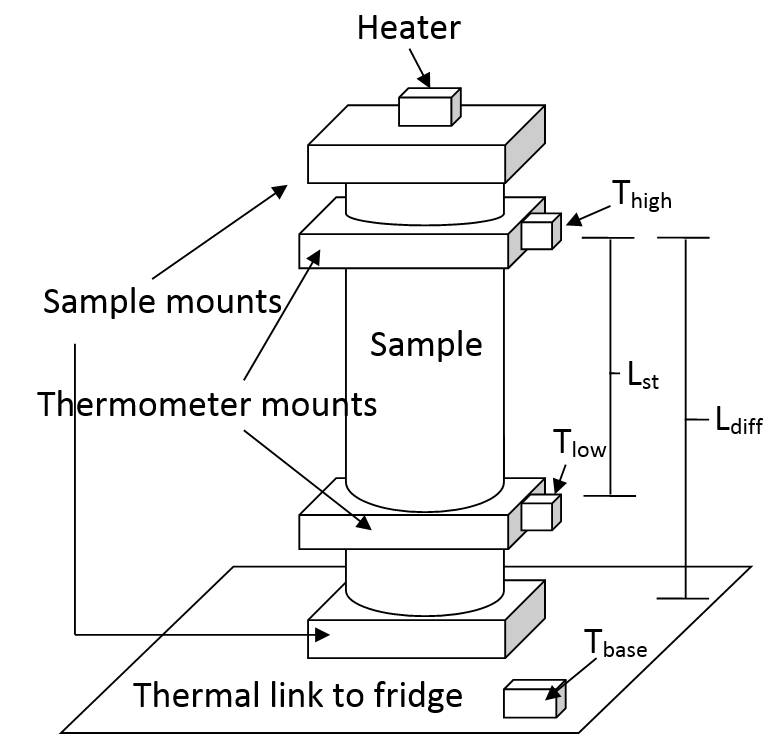
\includegraphics[width = .4\textwidth]{Rep_test_sample.png}
\qquad
\includegraphics[width = .272\textwidth]{kap_sample.png}
\includegraphics[width = 0.22\textwidth]{kapton_assembled.png}

\caption{{\small Left shows a representative test set-up for five of the seven thermal conductivity tests. Primarily two thermometers ($T_{high}$ and $T_{low}$) were used for measurements, but a third ($T_{base}$) was mounted on the fridge end to verify base temperatures. Middle shows the Kapton-epoxy and Ti 15-3-3-3 samples. They were folded back onto themselves numerous times and clamped with the thermometer mounts to give a large cross-section. Right shows the assembled sample with heater and fridge mounts at the ends and thermometer mounts in the middle. Flooding the dishes with epoxy ensures sufficient thermal contact so that the heat flow through the sample will be planar, and the gradient across the sample folds will be uniform. }}
\label{setup}
\end{figure}

\section{Experimental Configuration for Thermal Conductivity Tests}
The thermal conductivities of several materials were measured. All measurements were conducted in a $^3$He-$^4$He dilution refrigerator in the range of 0.05K - 1K, with the specific range varying depending on the material.

Figure \ref{setup} shows a representative test set-up for the thermal conductivity tests. A single heater was used to provide power; this was a 20k$\Omega$ metal film resistor for all tests except Vespel SP-22 and Vespel SCP-5050, which used a 2k$\Omega$ resistor. We read out temperatures with three thermometers, as shown in the figure. $T_{high}$ and $T_{low}$ were Ge thermistors, while $T_{base}$ was a RuO$_2$ thermistor, all from LakeShore\footnotemark. \footnotetext{www.lakeshore.com} A Keithley 213 Quad Voltage Source was used to read out the thermometers in a 4-wire configuration and to provide power to the heater. For temperatures above ~550mK, an LR-700 resistance bridge was used to read out the thermometers. $T_{high}$ and $T_{low}$ were each attached to individual copper clamp fixtures, separate from the heater/fridge mounts, to prevent any boundary resistance effects which could create a temperature measurement bias. Electrical connections used either 0.0012 inch or 0.003 inch diameter manganin wires -- depending on the sample -- all with lengths of $>$ 6 inches to the fridge thermal link. Finally, the sample was placed within a 50mK shield which prevented any radiative heat loads on the sample.

\begin{wraptable}{r}{6.0cm}
\centering
\small
\rowcolors{3}{gray!20}{white}
\begin{tabular}{rrr}
\toprule
\textbf{Material} & $L_{st}$ (cm) & Area (cm$^2$) \\\midrule
Vespel SP-22 & 3.62 & 1.27 \\
Vespel SCP-5000 & 2.22 & 1.30 \\
Vespel SCP-5050 & 3.62 & 1.30 \\
Ti 15-3-3-3 & 3.05 & 0.91 \\
Graphlite CFRP & 4.03 & 0.12 \\
2020 graphite & 1.42 & 12.97 \\
Kapton-epoxy & 3.05 & 1.17 \\
\bottomrule
\end{tabular}
\caption{{\small Length and cross-section for thermal conductivity samples. $L_{st}$ refers to the center-to-center thermometer separation.}}
\label{dim}
\end{wraptable}

Table \ref{dim} gives the dimensions for each sample tested. Every sample was a cylindrical rod with the exception of the Ti 15-3-3-3 and Kapton-epoxy, which were strips of material folded back on itself repeatedly then clamped with the thermometer mounts, as shown in the right side of Figure \ref{setup}. Copper mounts were glued to the ends of each sample using Hardman's Double-Bubble Epoxy for the Ti 15-3-3-3, Kapton-epoxy, and grade 2020 graphite, and Stycast 1266 for all other samples. The strip samples used copper dishes which were flooded with epoxy to contact the sample.

\section{Thermal Conductivity Measurement Methods}
The longitudinal heat flow method was used in all tests to determine thermal conductivity. We applied a heat load to the top of the sample and let it reach equilibrium, which established a temperature gradient along the sample; this took between 30-180 minutes depending on the sample and temperature range. Once in equilibrium, we relate power through the sample and K(T) with
\begin{equation}
P = P_{heater} + P_{parasitic} = \int_{T_{low}}^{T_{high}} \frac{A}{L_{st}} K(T)dT\\
\label{heat_flow}
\end{equation}
where A is the cross-section of the sample, $L_{st}$ is the sample length between the two thermometers, K(T) is the thermal conductivity of the sample, $P_{heater}$ is the power applied through the heater, and $P_{parasitic}$ is any other parasitic heat load through the sample (e.g. from wiring, voltage noise in the heater, etc.)

We primarily used two methods to determine thermal conductivity. The simplest method assumes a constant thermal conductivity\footnotemark \footnotetext{Depending on K(T), this assumption can be valid for gradients of $> 100$\% of $T_{avg}$. See \cite{Hust1982} for details.} along the gradient from $T_{high}$ to $T_{low}$. We bring thermal conductivity out of the integral, integrate with respect to T, and solve for K($T_{avg}$), where $T_{avg} = (T_{high} + T_{low})/2$. The second method assumes a parametric form for thermal conductivity -- this is often a power law at low temperatures ($K(T) = A \times T^B$). This lets us directly integrate equation \ref{heat_flow}. The free parameters are then varied to find the those values which minimize
\begin{eqnarray}
\chi^2 = \sum_{i = 1}^{n} \left[\frac{P_{total_i} - P_{expected_i}}{\sigma_{P_i}}\right]^2 \qquad ,
\label{param}
\end{eqnarray}
for n measurements, where $P_{total_i} = P_{heater_i} + P_{parasitic_i}$ is a combination of power applied to the heater and any parasitic heat loads, $P_{expected_i}$ is given by the right side of equation \ref{heat_flow}, and $\sigma_{P_i}$ is the total variance in power for a given measurement.

\section{Thermal Conductivity Results}
Measured thermal conductivities are shown on the left plot of Figure \ref{plots}. Error bars are given for the points obtained using the constant thermal conductivity approximation method. The black error bars give the measurement uncertainty, while the green regions give the combined measurement and systematic uncertainty. We also plot the parametric forms, given in Table \ref{cond_table}. The good agreement between the two methods demonstrates the validity of the constant thermal conductivity approximation. Overall errors in K(T) are estimated to be between 6\%-15\%, with the lowest temperature points being up to 20\%; these errors are heavily dominated by uncertainty in power through the sample -- especially from parasitic heat loads at low temperatures -- and on uncertainty in length for the sample, which was conservatively set to the length of the thermometer mount contact area.

\begin{wraptable}{r}{5.3cm}
\centering
\small
\begin{threeparttable}
\rowcolors{3}{gray!20}{white}
\begin{tabular}{lr}
\toprule
Sample & K(T) [uW/cm-K] \\
\midrule
2020 graphite & $7.88$ T$^{1.00}$ \\
Vespel SCP-5050 & $10.0$ T$^{1.98}$ \\
Vespel SCP-5000 & $13.8$ T$^{1.11}$ \\
Vespel SP-22 & $22.1$ T$^{2.15}$ \\
Ti 15-3-3-3 & $131.1$ T$^{2.10}$ \\
Graphlite & $160.0$ T$^{1.54}$ \\
Kapton-epoxy: & \\
\multicolumn{2}{r}{$10^{1.81 + 1.01log(T) - 0.348log^2(T)}$} \\
\bottomrule
\end{tabular}
\caption{{\small Parameterized K(T) measured for materials. Only the Kapton-epoxy did not follow a power-law.}}
\label{cond_table}
\end{threeparttable}
\end{wraptable}

The right side of Figure \ref{plots} compares our conductivity measurements to data in the literature. We see that the thermal conductivity of grade 2020 graphite is very similar to POCO AXM-5Q. In addition, both SCP-5000 and SCP-5050 have lower conductance than their counterparts SP-1 and SP-22, making them very interesting for experimental applications. Our measured thermal conductivity for Vespel SP-22 is lower than the results from J.R. Olson\cite{Olson1993}, and may be attributed to a large uncertainty in parasitic heat loads. Our results for Graphlite were higher than Runyan \& Jones' results\cite{Runyan2008}; the discrepancy could be due to the fact that their group did not test official Graphlite, but a very similar CFRP with the same fiber fill volume and bisphenol-based epoxy.  The values obtained for Kapton-epoxy are consistent with the literature as well, if we assume that the epoxy has higher thermal conductivity than Kapton. For Ti 15-3-3-3, although our results are consistent at high temperatures with those reported by Wikus et al.\cite{Wikus2010}, we do not observe the sharp drop in conductivity they report below 500mK; even so, its low thermal conductivity makes it useful for low conductance applications.

\begin{figure}[h]
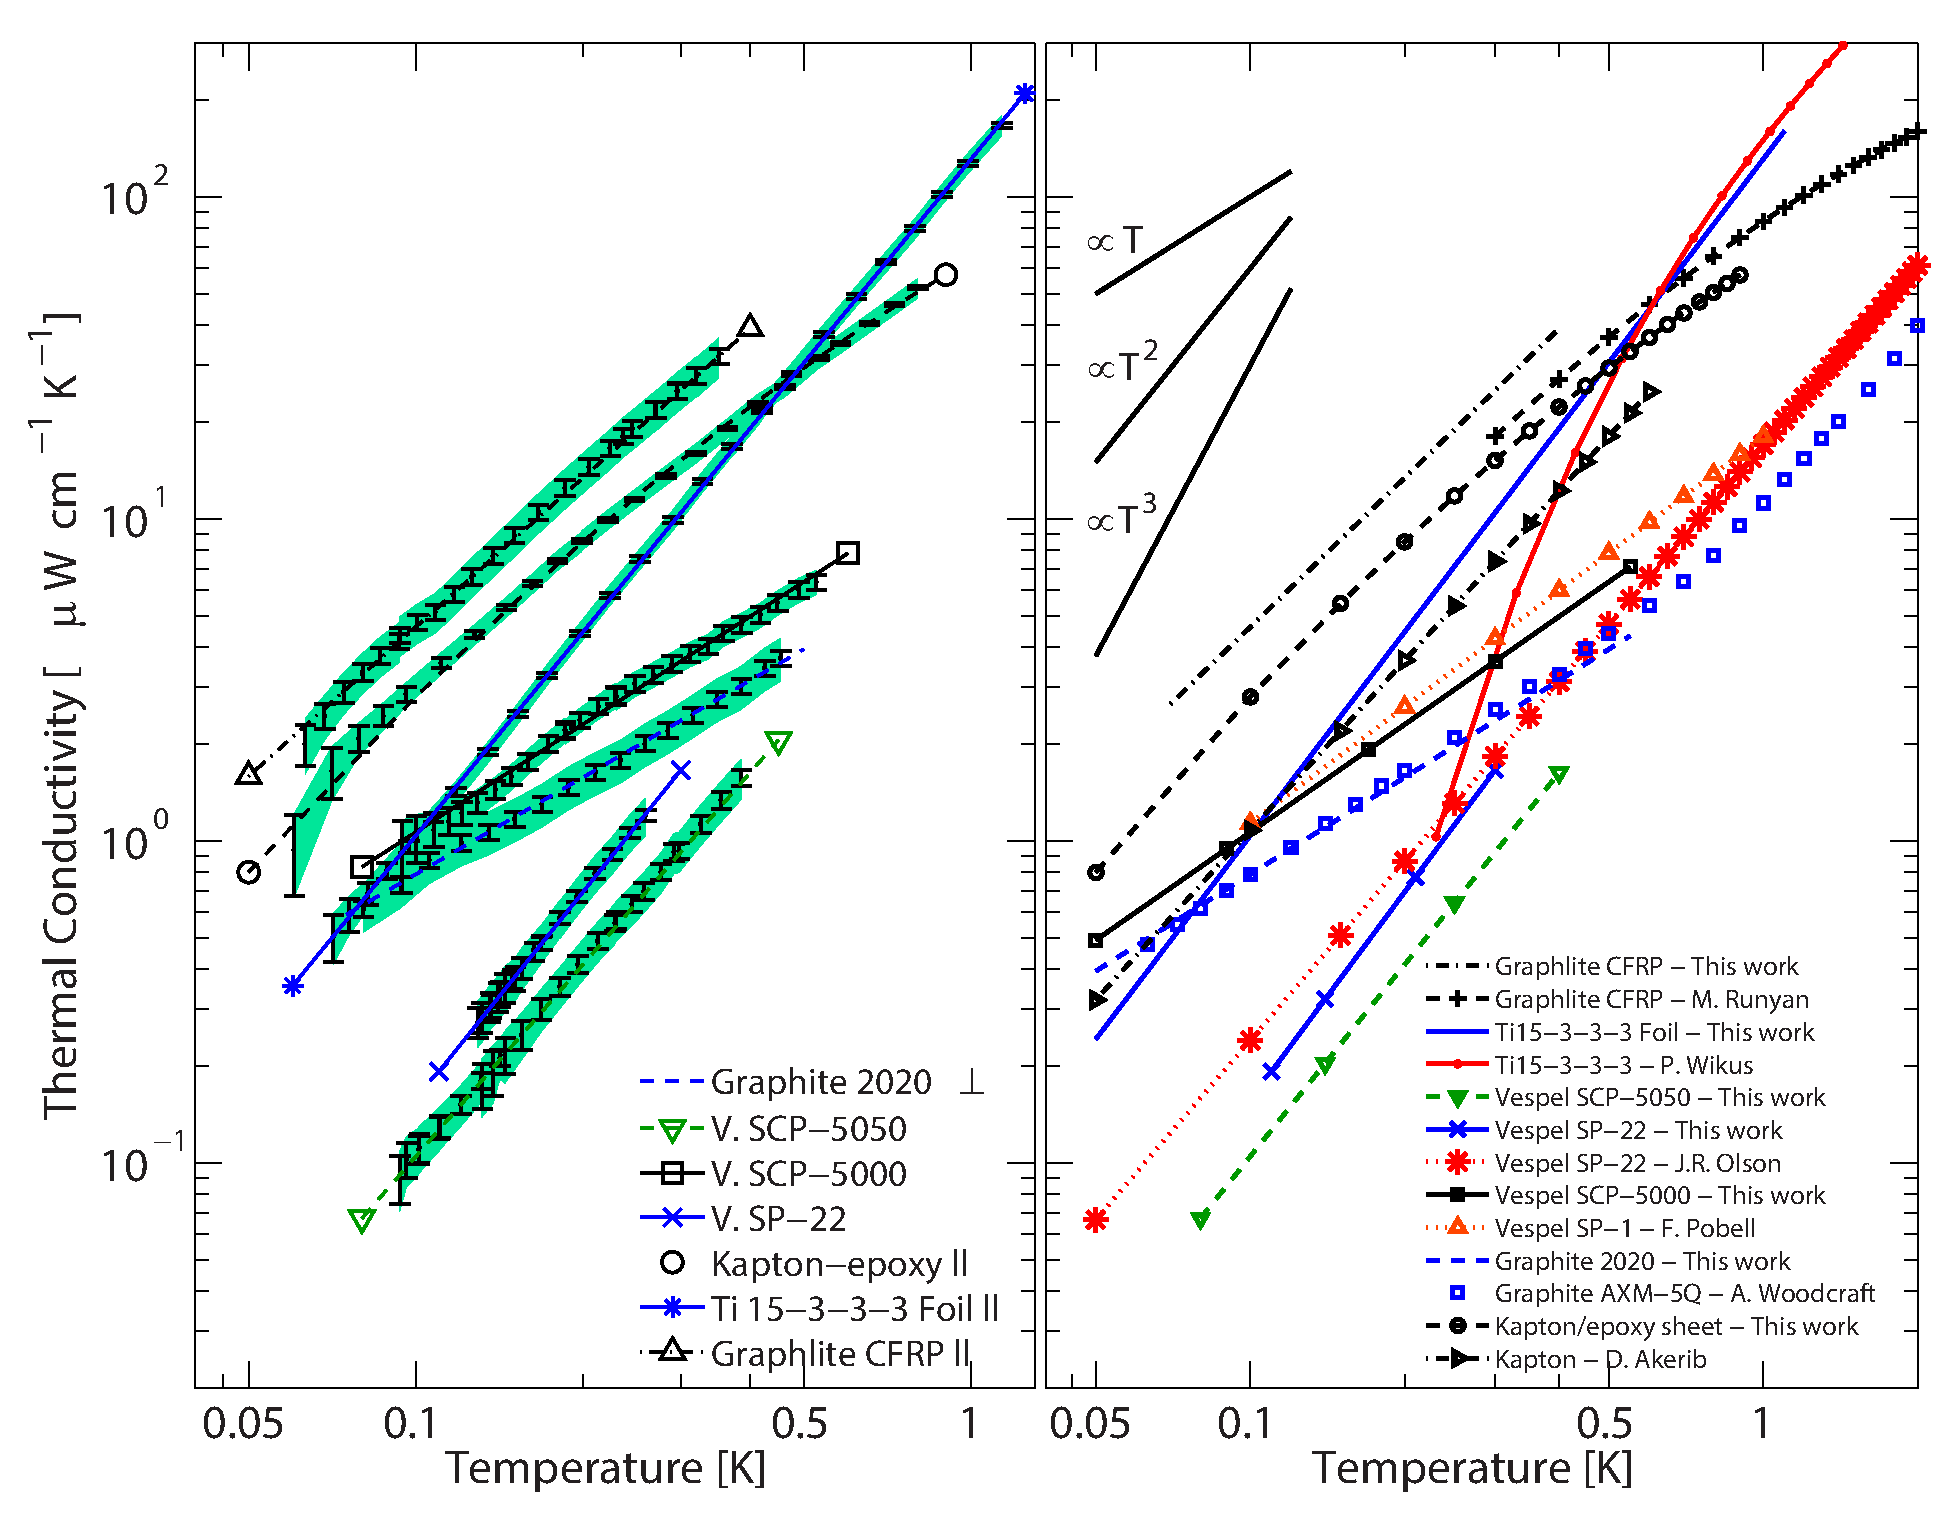
\includegraphics[width = 1\textwidth,trim = 0 0 0 0]{K_plots.eps}
\caption{{\small Thermal conductivity of tested materials compared to other materials of interest. In the left plot, black error bars give measurement uncertainty, while the green shading gives systematic + measurement uncertainty at 60\% CL. In the left legend, $\parallel$ signifies that Graphlite was measured parallel to the fiber axis, and Kapton-epoxy/Ti 15-3-3-3 were measured parallel to the plane of the sheet. $\perp$ denotes that 2020 was measured perpendicular to the grain orientation. In both plots, parametric forms are plotted for data from this work. All other data is from: Graphlite\cite{Runyan2008}, Ti 15-3-3-3\cite{Wikus2010}, Vespel SP-22\cite{Olson1993}, Vespel SP-1\cite{Pobell1992}, Graphite AXM-5Q\cite{Woodcraft2009}. The Kapton data is from an in-lab measurement by Dan Akerib in the CDMS collaboration. (color version online)}}
\label{plots}
\end{figure}

\noindent \textbf{Acknowledgements}

\noindent We would like to thank Curbell Plastics and Tech-Etch for donating samples for testing. This work was funded by the Department of Energy and the National Science Foundation.


\vspace{-0.41cm}

\begin{thebibliography}{99}

\bibitem{Hust1982}
J.G. Hust and A.B. Lankford, {\it Int. Journal of Thermophysics} \textbf{3}, 67, (1982).

\bibitem{Woodcraft2009}
A.L. Woodcraft, M. Barucci, P.R. Hastings, L. Lolli, V. Martelli, L. Risegari, and G. Ventura, {\it Cryogenics} \textbf{49}, 159, (2009).

\bibitem{Runyan2008}
M.C. Runyan and W.C. Jones, {\it Cryogenics} \textbf{48}, 448, (2008).

\bibitem{Wikus2010}
P. Wikus, S.A. Hertel, S.W. Leman, K.A. Mc{C}arthy, S.M. Ojeda, and E. Figueroa-{F}eliciano, {\it Cryogenics} \textbf{51}, 41, (2010).

\bibitem{Pobell1992}
F. Pobell, {\it Matter and Methods at Low Temperatures} (Springer--Verlag, Heidelberg, Germany, 1992)

\bibitem{Olson1993}
J.R. Olson, {\it Cryogenics} \textbf{33}, 729, (1993).

\end{thebibliography}

\end{document}
